\documentclass[9pt,xcolor=table]{beamer}
\usetheme{Warsaw}

\usepackage{tikz}
\usepackage{xcolor}
\usepackage{xltxtra}
\usepackage{dirtree}
\usepackage{ragged2e}
\usepackage{listings}
\usepackage{graphicx}
\usepackage{chronology}
\usetikzlibrary{shapes, arrows}

\lstset{
    language=Bash,
    backgroundcolor=\color{black!5},
    basicstyle=\footnotesize\ttfamily\color{black},
    keywordstyle=\color{blue},
    stringstyle=\color{red},
    commentstyle=\color{green!70!black},
    numbers=none,
    numberstyle=\tiny\color{gray},
    stepnumber=1,
    numbersep=5pt,
    showspaces=false,
    showstringspaces=false,
    showtabs=false,
    frame=single,
    rulecolor=\color{black},
    tabsize=2,
    captionpos=b,
    breaklines=true,
    breakatwhitespace=false,
    escapeinside={\%*}{*)},
    morekeywords={*,...}
}

\date{20 de maio de 2023}
\title{OpenBSD: Segurança e Inovação em SOs}
\institute[PUC]{Pontifícia Universidade Católica de Minas Gerais}
\logo{
\includegraphics[width=0.7cm]{imagens/logo_pucminas.png}}
\author[Gustavo Valadares, Hernane Rosa, João Víctor, Pedro Igor]{Gustavo Valadares \and Hernane Rosa \and João Martins \and Pedro Igor}

\begin{document}

\begin{frame}
  \titlepage
\end{frame}
\begin{frame}{Introdução}
  \begin{itemize}
    \item O que é o OpenBSD?
    \item Breve histórico do projeto;
    \item Objetivos do OpenBSD.
  \end{itemize}
\end{frame}
\begin{frame}{O que é o OpenBSD?}
  \begin{itemize}
    \item OpenBSD é um sistema operacional livre e de código aberto baseado no ramo BSD.
    \item Destaca-se por sua ênfase em segurança, portabilidade e código limpo.
    \item Desenvolvido desde 1995 por uma comunidade global liderada por Theo de Raadt.
    \item Utiliza uma licença permissiva (licença BSD), permitindo modificações e distribuição livre.
    \item Amplamente adotado em servidores, roteadores, estações de trabalho e dispositivos embarcados.
  \end{itemize}
\end{frame}
\begin{frame}{O que é o OpenBSD?}
    \begin{columns}
        \begin{column}{0.3\textwidth}
            \begin{figure}
            \centering
            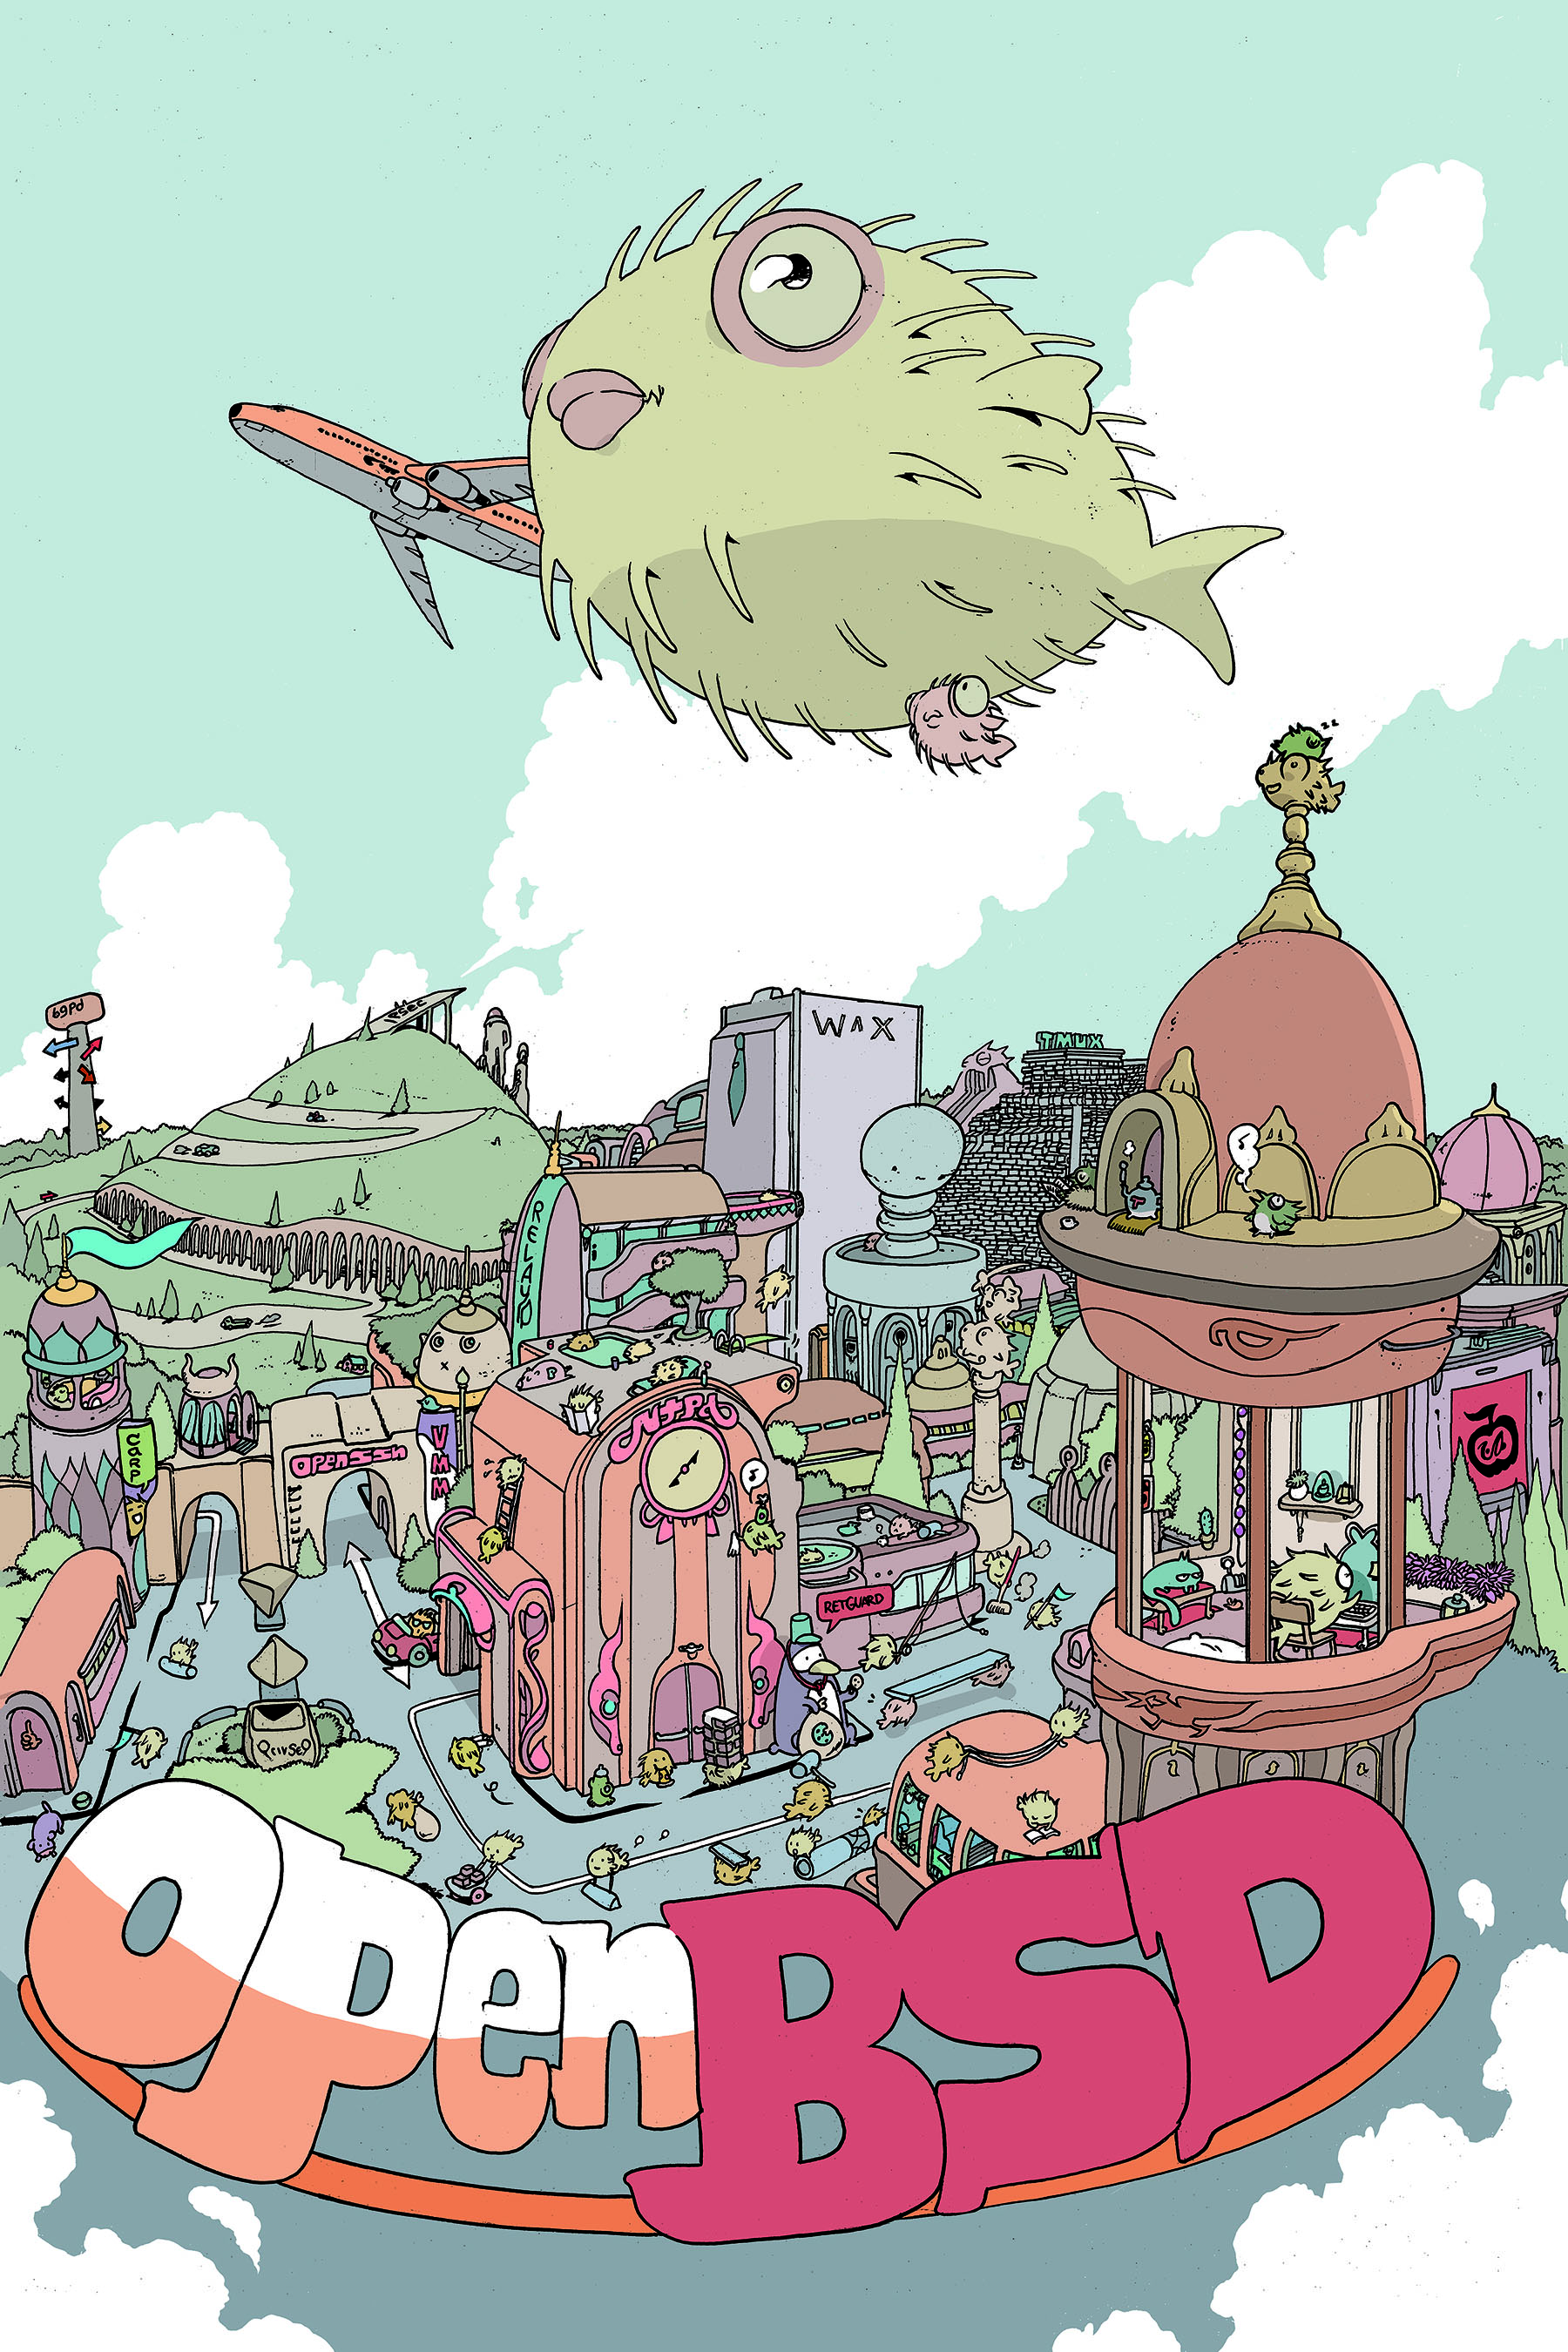
\includegraphics[width=\textwidth]{imagens/openbsd-fan.jpg}
            \caption{\textit{Fanart}}
            \end{figure}
        \end{column}
        \begin{column}{0.3\textwidth}
            \begin{figure}
            \centering
            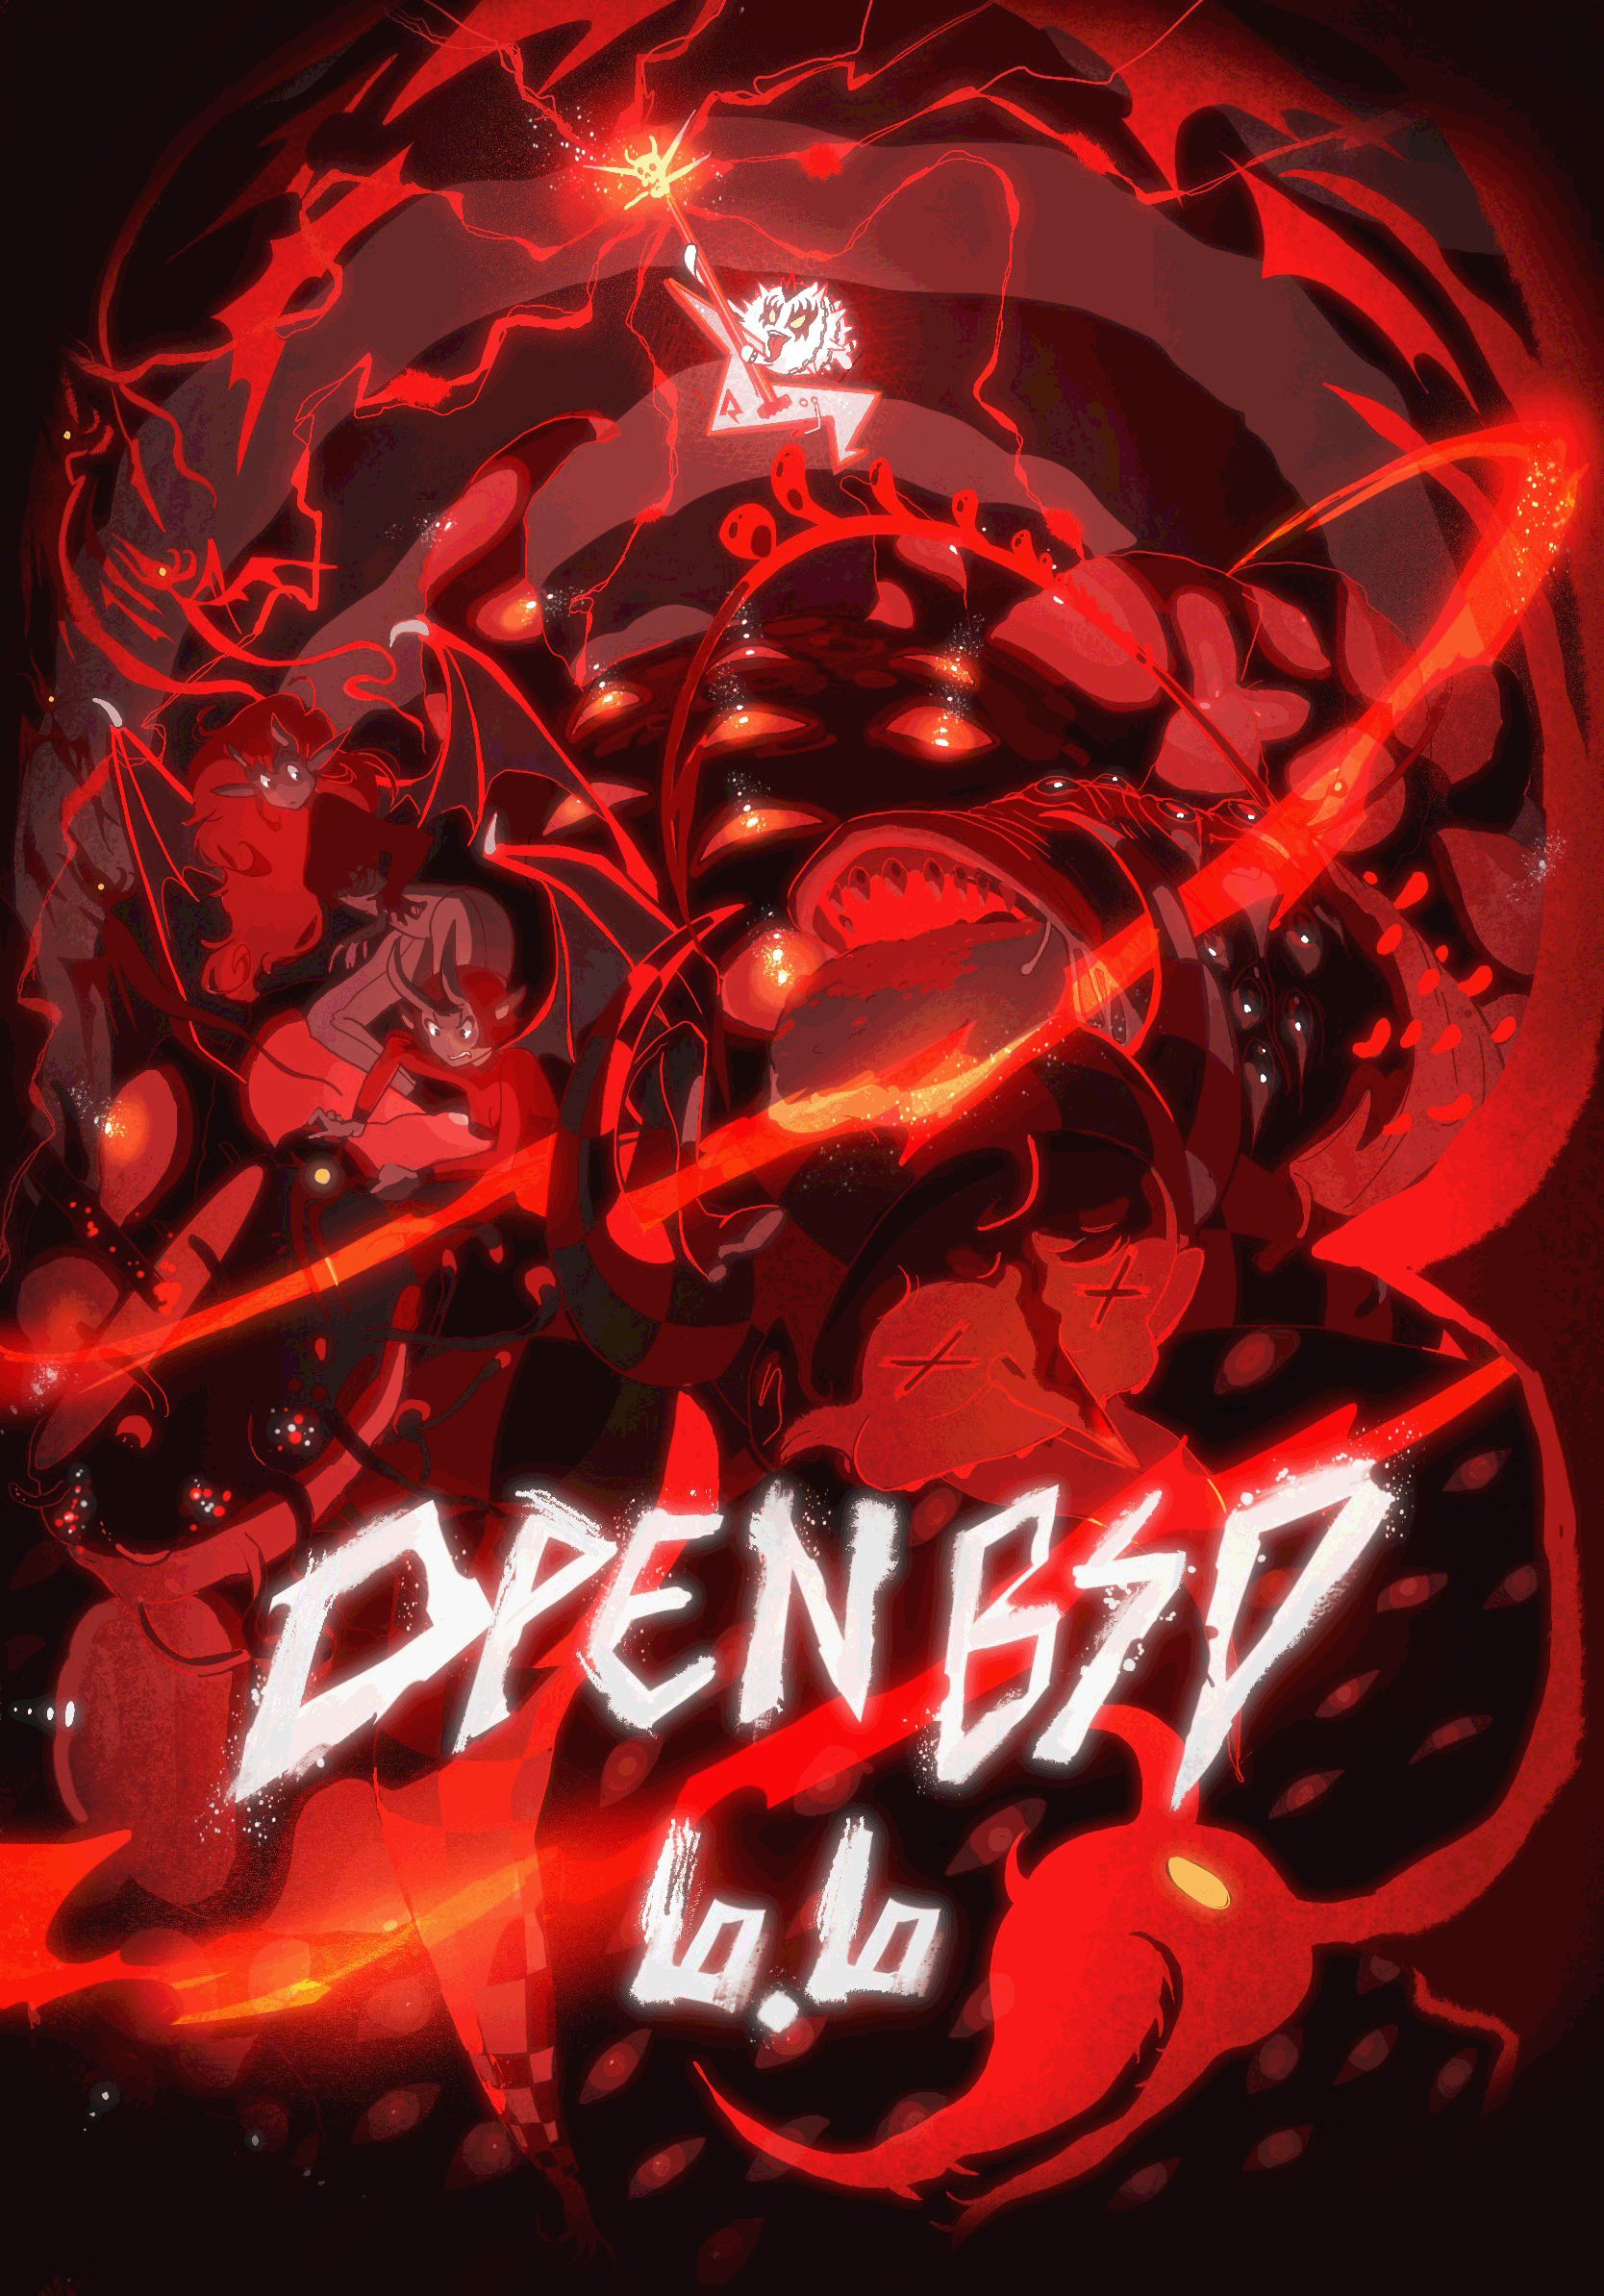
\includegraphics[width=\textwidth]{imagens/banner-openbsd.png}
            \caption{Pôster}
            \end{figure}
        \end{column}
        \begin{column}{0.3\textwidth}
            \begin{figure}
            \centering
            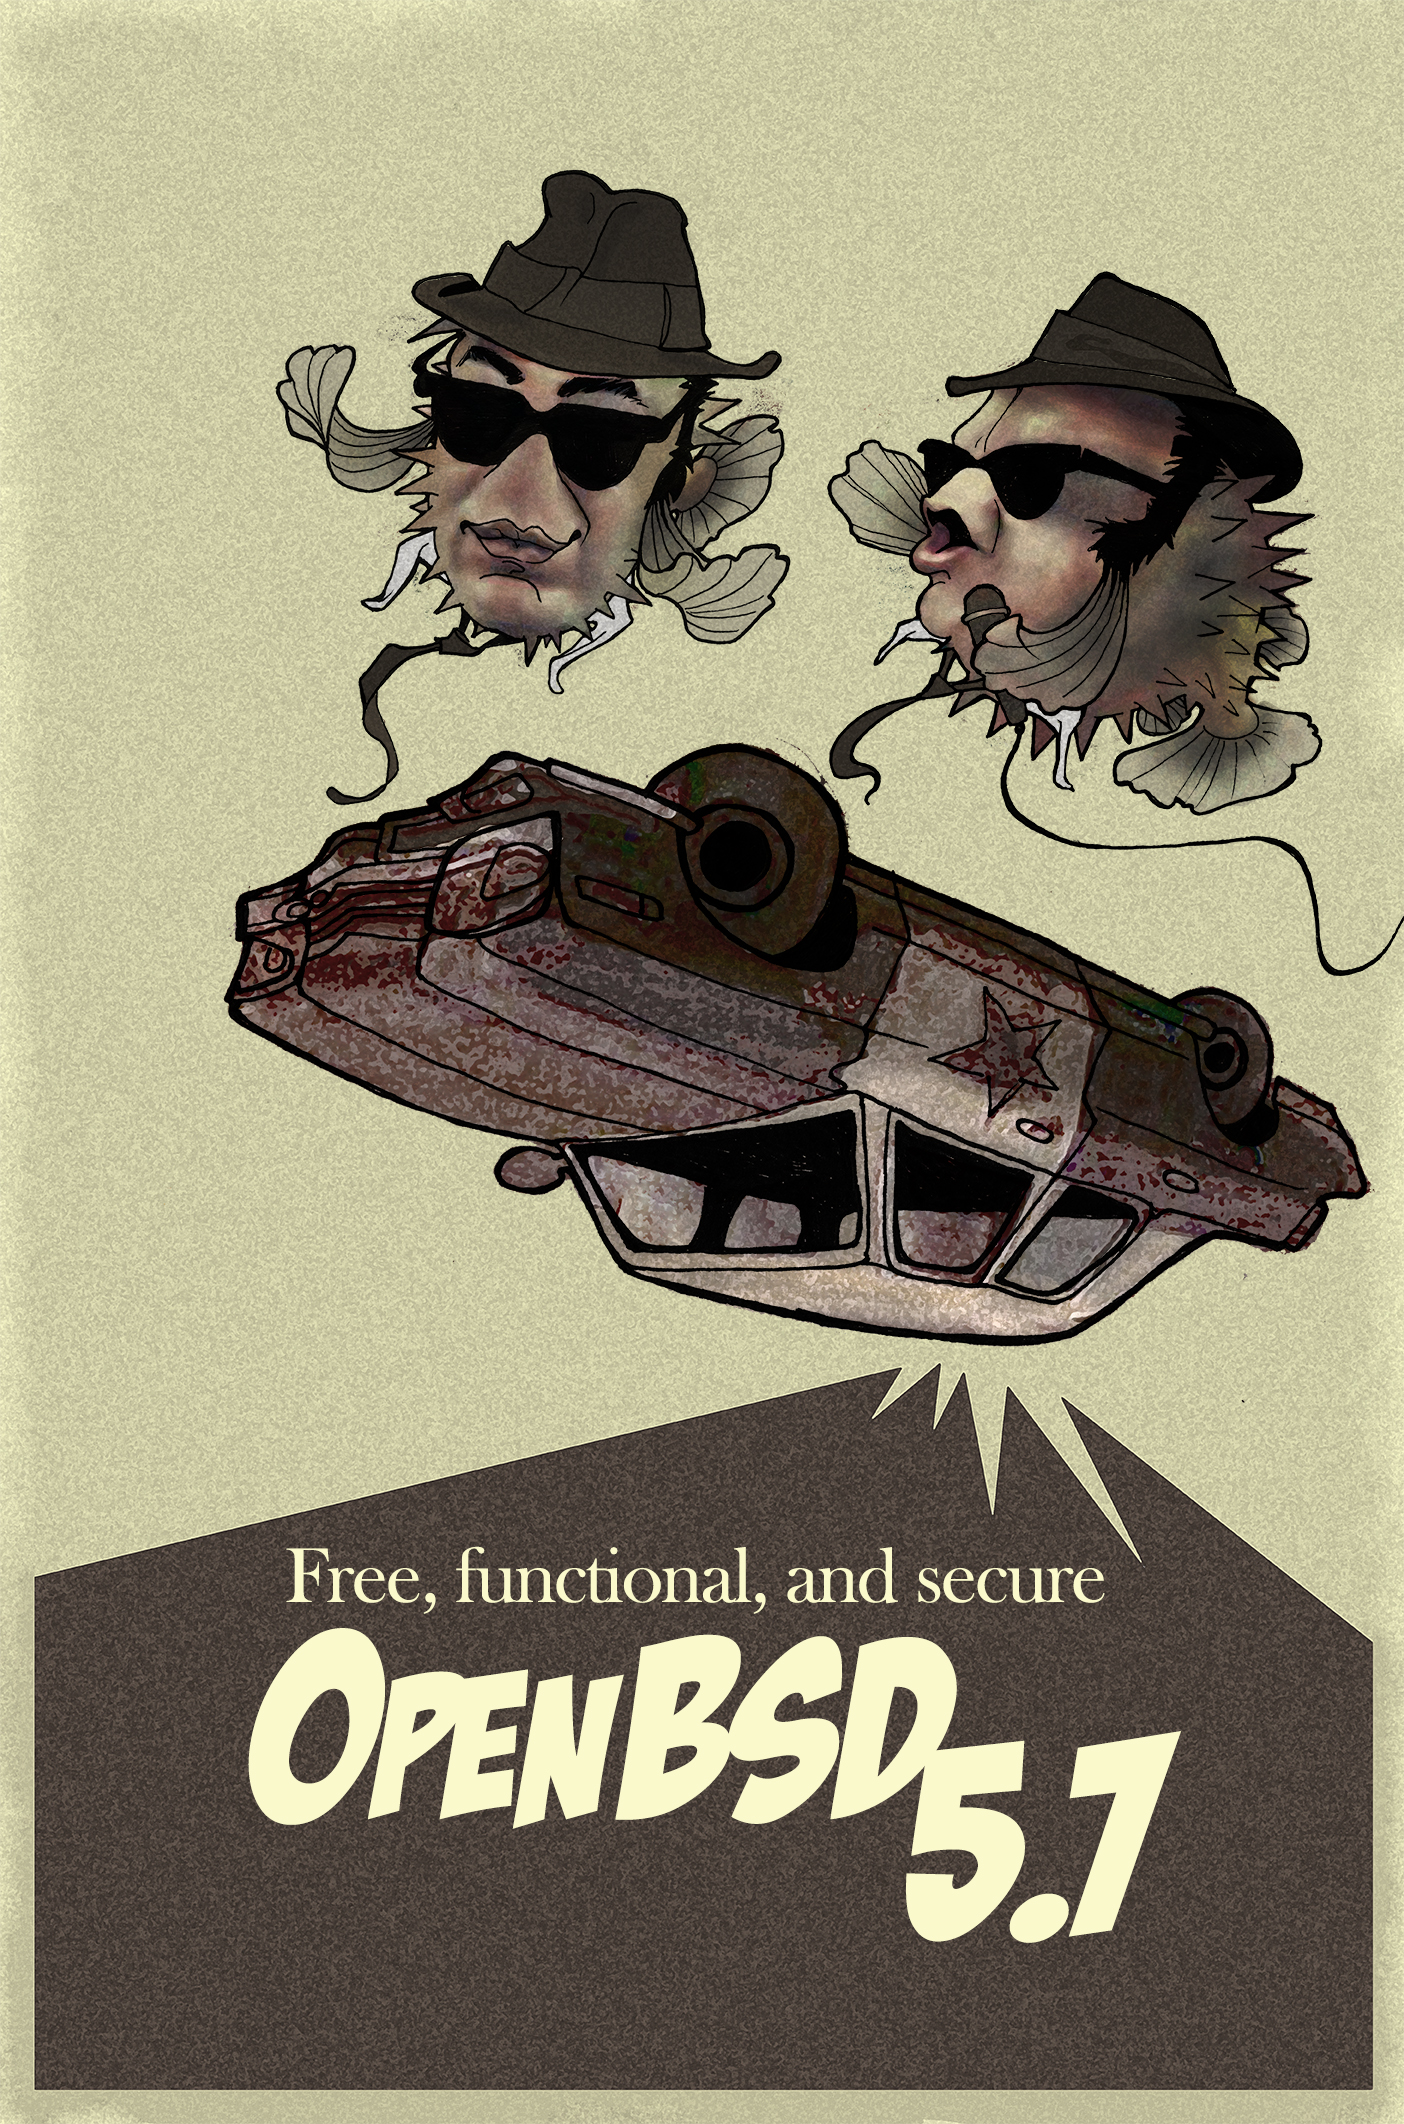
\includegraphics[width=\textwidth]{imagens/openbsd-poster.jpg}
            \caption{Capa de DVD}
            \end{figure}
        \end{column}
    \end{columns}
\end{frame}
\begin{frame}
\frametitle{Instalação do OpenBSD}
\begin{figure}
\centering
\begin{tikzpicture}[node distance = 3cm, auto]

\tikzstyle{startstop} = [rectangle, rounded corners, text centered, draw=black, fill=orange!30]
\tikzstyle{process} = [rectangle, text centered, draw=black, fill=blue!20]
\tikzstyle{decision} = [diamond, text centered, draw=black, fill=green!30]
\tikzstyle{error} = [trapezium, draw, text centered, trapezium left angle=60, trapezium right angle=120, fill=red!10]
\tikzstyle{arrow} = [thick,->,>=stealth]

\node (start) [startstop] {ISO};
\node (media) [process, right of=start] {Mídia USB};
\node (boot) [decision, below of=media] {Boot};
\node (inst) [startstop, left of=boot] {Instalação};
\node (config) [process, left of=inst] {Configuração};
\node (finish) [process, above of=config] {Fim};
\node (erro) [error, below of=boot] {Erro};

\draw [arrow] (start) -- (media);
\draw [arrow] (media) -- (boot);
\draw [arrow] (config) -- (finish);
\draw [arrow] (boot) -- (inst);
\draw [arrow] (inst) -- (config);
\draw [arrow,dashed] (inst) -- (erro);
\draw [arrow,dashed] (erro) -- (boot);
\end{tikzpicture}
\end{figure}
\end{frame}
\begin{frame}{História do OpenBSD}
\begin{chronology}[5]{1995}{2022}{\textwidth}
\event[1995]{1995}{Início do desenvolvimento}
\event[1997]{1997}{OpenBSD Ports}
\event[1999]{1999}{OpenSSH}
\event[2002]{2002}{OpenNTPD}
\event[2005]{2005}{Sshguard}
\event[2012]{2012}{OpenBSD Foundation}
\event[2015]{2015}{LibreSSL}
\event[2020]{2020}{OpenRSYNC}
\end{chronology}
\end{frame}
\begin{frame}[fragile]
\frametitle{Gerenciamento Seguro de Usuários no OpenBSD}
\justifying
O gerenciamento de usuários é semelhante aos demais sistemas operacionais Unix, ou seja, é possível determinar nome, \verb|groups|, ID, permissões, regras de pastas etc.
\begin{lstlisting}
root@openbsd > $ useradd -m pigor               # Criação.
root@openbsd > $ passwd                         # Alterar senha.
root@openbsd > $ usermod -c "Pedro Igor" pigor  # Atualizar informações.
root@openbsd > $ id pigor                       # Imprimir informações.
root@openbsd > $ userdel pigor                  # Remoção
\end{lstlisting}
\end{frame}

\begin{frame}[fragile]
\frametitle{Introdução ao OpenBSD Ports}
\justifying
O sistema de Ports do OpenBSD é uma ferramenta poderosa que simplifica a instalação de software de terceiros. Ele permite que os usuários instalem e atualizem aplicativos de maneira fácil e eficiente.
\vspace{0.5cm}
\begin{lstlisting}
$ cd /tmp
$ ftp https://cdn.openbsd.org/pub/OpenBSD/$(uname -r)/{ports.tar.gz,SHA256.sig}
$ signify -Cp /etc/signify/openbsd-$(uname -r | cut -c 1,3)-base.pub -x SHA256.sig ports.tar.gz
\end{lstlisting}
\end{frame}
\begin{frame}[fragile]
\frametitle{Estrutura e Uso dos Ports}
\justifying
Cada \textbf{port} é essencialmente um conjunto de metadados que descreve como baixar, descompactar, corrigir, compilar e instalar um aplicativo. O diretório de ports (\verb|/usr/ports|) contém uma subpasta para cada aplicativo disponível.
\vspace{0.5cm}
\dirtree{%
.1 /usr/ports.
.2 net.
.3 rsnapshot.
.4 Makefile.
.4 distinfo.
.4 patches.
.4 files.
.4 pkg.
.4 README.
.3 \ldots.
}
\end{frame}
\begin{frame}[fragile]
\frametitle{Estrutura e Uso dos Ports}
\justifying
Para instalar um aplicativo usando ports, você navega até a subpasta correspondente e executa \verb|make install|. Isso baixará o código-fonte do aplicativo, aplicará quaisquer patches necessários, compilará o código-fonte e instalará o aplicativo.
\vspace{0.5cm}
\begin{lstlisting}
$ make install
===>  Checking files for rsnapshot-1.4.2
>> Fetch https://github.com/rsnapshot/rsnapshot/archive/1.4.2/rsnapshot-1.4.2.tar.gz
100% |**************************************************|   365 KB    00:02
>> (SHA256) rsnapshot-1.4.2.tar.gz: OK
===> rsnapshot-1.4.2 depends on: metaauto-* - not found
[...]
===>  Installing rsnapshot-1.4.2 from /build/source/ports/packages/amd64/all/
rsnapshot-1.4.2: ok
\end{lstlisting}
\end{frame}
\begin{frame}
\frametitle{Importância dos Ports}
\justifying
Os Ports são uma parte essencial do ecossistema OpenBSD. Eles permitem que os usuários se beneficiem de uma ampla gama de software de terceiros, sem a necessidade de rastrear e compilar o código-fonte manualmente. Além disso, como o sistema de Ports cuida de todas as dependências, ele garante que cada aplicativo funcione corretamente após a instalação.
\vspace{0.5cm}
\begin{columns}
\begin{column}{0.3\textwidth}
\begin{figure}
\centering

\includegraphics[width=0.5\textwidth]{imagens/hydra-logo.png}
\caption{Hydra}
\end{figure}
\end{column}
\begin{column}{0.3\textwidth}
\begin{figure}
\centering

\includegraphics[width=0.5\textwidth]{imagens/mpv-logo.png}
\caption{MPV}
\end{figure}
\end{column}
\begin{column}{0.3\textwidth}
\begin{figure}
\centering

\includegraphics[width=0.5\textwidth]{imagens/kde-logo.png}
\caption{KDE Plasma}
\end{figure}
\end{column}
\end{columns}
\end{frame}
\begin{frame}[fragile]
\frametitle{Introdução ao OpenSSH}
\textbf{OpenSSH} (\textit{Open Secure Shell}) é um conjunto de ferramentas de conectividade de computador que fornecem criptografia de comunicações em uma rede de computadores. Ele foi criado como um projeto do OpenBSD e é padrão em muitos sistemas operacionais Unix-like.
\vspace{0.5cm}
\begin{lstlisting}
pigor@gigabyte > $ ssh root@192.168.1.9
root@192.168.1.9`s password:
[....]
root@192.168.1.9 > #
\end{lstlisting}
\end{frame}
\begin{frame}[fragile]
\frametitle{OpenNTPD}
\justifying
\textbf{OpenNTPD} é uma implementação simples e segura do Protocolo de Tempo de Rede (\textit{Network Time Protocol - NTP}). Foi desenvolvido como parte do projeto OpenBSD com o objetivo de ser tão seguro, fácil de usar e livre de bugs quanto possível.
\vspace{0.5cm}
\begin{lstlisting}
$ grep ntpd /var/log/daemon.log | grep adjusting
May 10 03:32:20 pigor ntpd[4784]: adjusting local clock by -1.162333s
May 10 03:36:08 pigor ntpd[4784]: adjusting local clock by -1.023899s
May 10 03:40:02 pigor ntpd[4784]: adjusting local clock by -0.902637s
May 10 03:43:43 pigor ntpd[4784]: adjusting local clock by -0.789431s
\end{lstlisting}
\end{frame}
\begin{frame}{Princípios do OpenBSD}
  \begin{itemize}
    \item Segurança como prioridade
    \item Código limpo e revisões extensivas
    \item Acesso aberto e colaborativo
    \item Documentação abrangente
  \end{itemize}
\end{frame}
\begin{frame}{Recursos de Segurança}
  \begin{itemize}
    \item Modelo de desenvolvimento e revisões de código;
    \item Análise de segurança proativa;
    \item Mecanismos de mitigação de ataques;
    \item Uso do OpenSSH como padrão;
    \item Política padrão "secure by default".
  \end{itemize}
\end{frame}
\begin{frame}
\frametitle{Introdução à "Segurança por padrão"}
\justifying
A política de \textbf{Segurança por padrão} do OpenBSD significa que, na instalação padrão, todos os serviços não essenciais serão desativados. O sistema operacional é configurado para ser seguro "fora da caixa", reduzindo a área de ataque e protegendo os usuários contra ameaças de segurança.
\vspace{0.5cm}
\begin{enumerate}
 \item W\^{}X;
 \item Address Space Layout Randomization;
 \item ProPolice (uma proteção de estouro de buffer).
\end{enumerate}
\end{frame}
\begin{frame}[fragile]
\frametitle{ASLR}
\justifying
\textbf{Address Space Layout Randomization} (\textit{ASLR}) é uma técnica de segurança que evita alguns tipos de ataques, como ataques de execução de código e estouro de buffer. Ele faz isso ao randomizar o layout do espaço de endereços de um processo, tornando mais difícil para um atacante prever o local de um determinado pedaço de código.
\vspace{0.5cm}
\begin{lstlisting}[language=C]
int global_variable = 42;

int main() {
    int local_variable = 123;
    printf("Endereço da variável global: %p\n", &global_variable);
    printf("Endereço da variável local: %p\n", &local_variable);
    return 0;
}
\end{lstlisting}
\end{frame}
\begin{frame}[fragile]
\frametitle{ASLR}
\justifying
A variável global chamada \verb|global_variable| e uma variável local chamada \verb|local_variable|. O programa imprime os endereços de memória dessas variáveis usando o especificador de formato \verb|%p| da função \verb|printf()|.

\begin{lstlisting}
$ gcc -o aslr_example aslr_example.c
$ ./aslr_example                              # 1ª Tentativa
Endereço da variável global: 0x7f7ce5a19034
Endereço da variável local: 0x7ffeb330ca1c
\end{lstlisting}
\vspace{0.1cm}
Ao compilar e executar esse código no OpenBSD, você verá que os endereços de memória das variáveis serão diferentes a cada execução. Isso ocorre porque o ASLR está em ação, randomizando a localização das variáveis na memória.
\begin{lstlisting}
$ ./aslr_example                              # 2ª Tentativa
Endereço da variável global: 0x7f4ed2923034
Endereço da variável local: 0x7ffedc9db81c
\end{lstlisting}
\end{frame}
\begin{frame}[fragile]
\frametitle{W\^{}X}
\justifying
OpenBSD implementa a política \textbf{W\^{}X} por padrão. Isso significa que, por padrão, todas as páginas de memória no sistema são configuradas para serem ou graváveis ou executáveis, mas nunca ambas. Esta política é implementada em todos os níveis do sistema, desde o kernel até os aplicativos de espaço do usuário.
\vspace{0.5cm }
\begin{lstlisting}[language=C]
void function() {
    printf("Esta é uma função protegida pelo W^X.\n");
    char* writable_memory = (char*)function;
    writable_memory[0] = 'X';
}

int main() {
    void (*function_ptr)() = &function;
    function_ptr();
    return 0;
}
\end{lstlisting}

\end{frame}
\begin{frame}[fragile]
\frametitle{ProPolice}
\justifying
\textbf{ProPolice} é uma extensão do compilador GCC que ajuda a prevenir estouros de buffer, um tipo comum de vulnerabilidade de segurança. Faz isso rearranjando a pilha de memória para tornar mais difícil para um atacante sobrescrever os dados importantes.
\vspace{0.5cm}
\begin{lstlisting}[language=C]
void vulnerable_function(char* input) {
    char buffer[10];
    strcpy(buffer, input);
    printf("Buffer: %s\n", buffer);
}

int main() {
    char input[20];
    printf("Digite um texto: ");
    fgets(input, sizeof(input), stdin);
    vulnerable_function(input);
    return 0;
}
\end{lstlisting}
\end{frame}
\begin{frame}[fragile]
\frametitle{ProPolice}
\justifying
A função chamada \verb|vulnerable_function| que copia o conteúdo da entrada do usuário para um buffer local sem verificar o tamanho do input. Isso pode levar a um estouro de pilha se o usuário fornecer uma entrada maior do que o tamanho do buffer.
\begin{lstlisting}
user@openbased > $ gcc -fstack-protector -o propolice_example
\end{lstlisting}
O OpenBSD compila o código com a opção de compilador \verb|-fstack-protector|, que adiciona um mecanismo de proteção ao estouro de pilha. Quando ativado, esse mecanismo verifica se o estouro de pilha ocorreu antes de permitir que a função retorne. Se o estouro de pilha for detectado, o programa será encerrado imediatamente.
\begin{lstlisting}
user@openbased > $ ./propolice_example
Digite um texto: Hello, Propolice!
Buffer: Hello, Prop
\end{lstlisting}
\end{frame}
\begin{frame}[fragile]
\frametitle{ProPolice}
Como dito, a \verb|string| continha apenas 10 caracteres e, por proteção, o programa será encerrado após violar o limite determinado.
\vspace{0.5cm}
\begin{table}[]
\begin{tabular}{|cccccccccc
>{\columncolor[HTML]{FFFC9E}}c
>{\columncolor[HTML]{FFFC9E}}c
>{\columncolor[HTML]{FFFC9E}}c
>{\columncolor[HTML]{FFFC9E}}c
>{\columncolor[HTML]{FFFC9E}}c
>{\columncolor[HTML]{FFFC9E}}c|}
\hline
H & e & l & l & o & , & P & r & o & p & \textbf{o}                & \textbf{l}                & \textbf{i}                & \textbf{c}                & \textbf{e}                & \textbf{!}                \\ \hline
0 & 1 & 2 & 3 & 4 & 5 & 6 & 7 & 8 & 9 & {\color[HTML]{FE0000} 10} & {\color[HTML]{FE0000} 11} & {\color[HTML]{FE0000} 12} & {\color[HTML]{FE0000} 13} & {\color[HTML]{FE0000} 14} & {\color[HTML]{FE0000} 15} \\ \hline
\end{tabular}
\end{table}
\end{frame}
\begin{frame}[fragile]
\frametitle{Gerenciamento de Memória no OpenBSD}
\begin{itemize}
\justifying
\item \textbf{Gerenciamento de memória unificado:} O OpenBSD usa um modelo de gerenciamento de memória unificado, tratando a memória física e virtual como um recurso unificado.

\item \textbf{Páginas de memória:} A memória é dividida em páginas, cada uma normalmente com 4 KB. Essas, por sua vez,  podem ser atribuídas a processos, usadas para armazenamento em buffer de I/O ou mantidas como páginas livres.

\item \textbf{Swapping e paging:} Quando a memória física fica baixa, o sistema pode mover páginas de memória inativas para o disco, um processo conhecido como \textit{swapping}. O OpenBSD também suporta \textit{paging}, que permite que partes de um processo sejam movidas para o disco para liberar memória.
\end{itemize}
\end{frame}
\begin{frame}[fragile]
\frametitle{Gerenciamento de Memória no OpenBSD}
\begin{itemize}
 \item \textbf{Monitorando o uso de memória:} Os comandos \verb|top|, \verb|vmstat| e \verb|systat| podem ser usados para monitorar o uso de memória no OpenBSD.
\begin{figure}
  \centering
  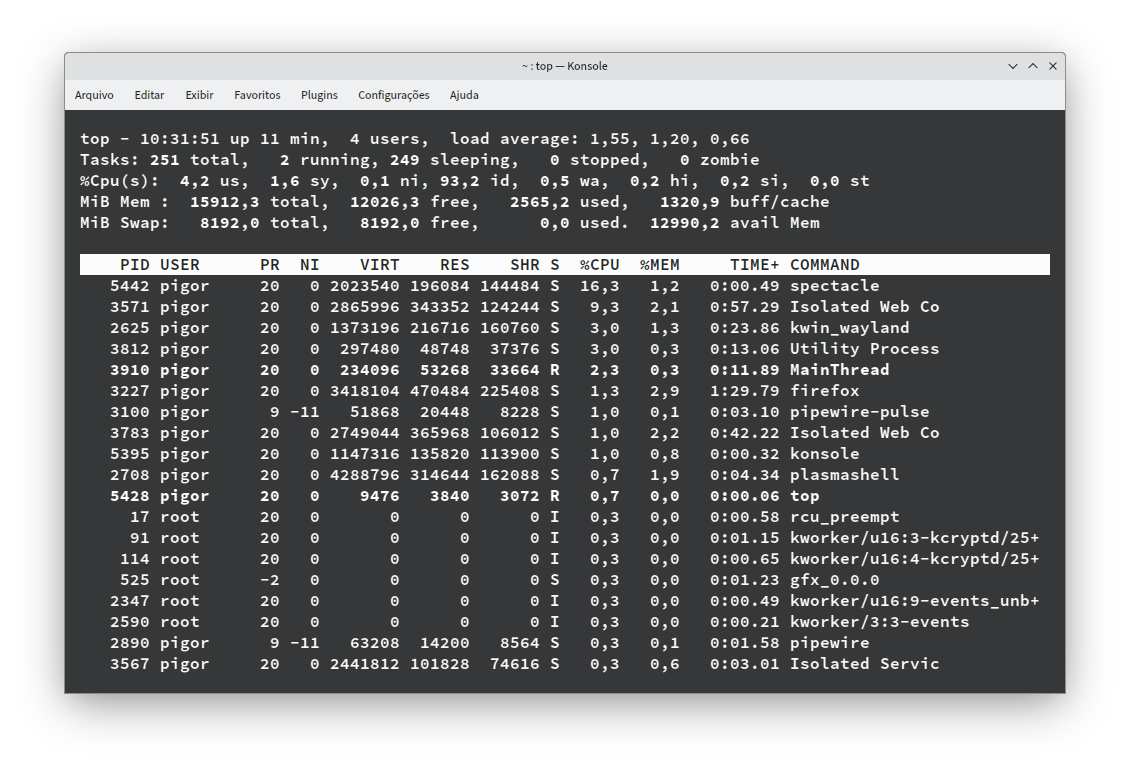
\includegraphics[width=0.8\textwidth]{imagens/screenshoot.png}
  \caption{Comando \textbf{top} em execução}
\end{figure}
\end{itemize}
\end{frame}
\begin{frame}[fragile]
\frametitle{Gerenciamento de Processos no OpenBSD}
\justifying
\begin{itemize}
\item \textbf{Iniciando processos:} Um processo é iniciado sempre que um programa é executado. Isso pode ser feito a partir da linha de comando ou como parte da inicialização do sistema.

\item \textbf{Prioridade de processos:} Utiliza um agendador de processos para determinar a ordem em que os processos são executados. A prioridade de um processo pode ser ajustada usando o comando \verb|nice| ou \verb|renice|.

\item \textbf{Segurança de processos:} Implementa vários mecanismos de segurança para processos, incluindo a execução de serviços em modos privilegiados mínimos e a separação de processos usando chroot ou outras técnicas de contenção.
\end{itemize}
\end{frame}
\begin{frame}
\frametitle{Sistemas de Arquivos no OpenBSD}

\begin{itemize}
\item \textbf{FFS}$_{2}$ (\textit{Enhanced Fast File System}): Este é o sistema de arquivos padrão usado pelo OpenBSD (6.7 >). É um sistema de arquivos Unix tradicional, otimizado para desempenho e confiabilidade.

\item \textbf{ext2/ext3/ext4:} Embora principalmente associados ao Linux, esses sistemas de arquivos também são suportados pelo OpenBSD, permitindo a interoperabilidade com sistemas Linux.

\item \textbf{FAT (File Allocation Table):} o sistema de arquivos FAT e sua variante VFAT, comumente usados em dispositivos USB e em sistemas Windows.

\item \textbf{NTFS (New Technology File System):} comumente usados em sistemas Windows mais recentes.

\item \textbf{CD9660 (ISO 9660):} Este é o sistema de arquivos padrão usado para CDs e DVDs.

\item \textbf{Outros sistemas de arquivos:} O OpenBSD também suporta uma variedade de outros sistemas de arquivos, incluindo UFS, NFS, SMBFS (para compartilhamentos de arquivos SMB/CIFS) e outros.
\end{itemize}
\end{frame}
\begin{frame}[fragile]
\frametitle{Sistemas de Arquivos no OpenBSD}
\begin{lstlisting}[caption=Partições padrão do OpenBSD]
16 partitions:
#       Size         Offset     Wfstype   [fsize bsize  cpg]
a:      2097121      64         7.3BSD      2048 16384    1 # /
b:      4698424      2097185    swap                        # swap
c:      312581808    0          unused
d:      8388576      6795617    7.3BSD      2048 16384    1 # /tmp
e:      16736864     15184193   7.3BSD      2048 16384    1 # /var
f:      4194304      31921057   7.3BSD      2048 16384    1 # /usr
g:      2097152      36115361   7.3BSD      2048 16384    1 # /usr/X11R6
h:      20971520     38212513   7.3BSD      2048 16384    1 # /usr/local
i:      4194304      59184033   7.3BSD      2048 16384    1 # /usr/src
j:      4194304      63378337   7.3BSD      2048 16384    1 # /usr/obj
k:      245003968    67572641   7.3BSD      2048 16384    1 # /home
\end{lstlisting}
\end{frame}
\begin{frame}{Recursos de Inovação}
  \begin{itemize}
    \item Virtualização com o VMM;
    \item Ferramentas e utilitários exclusivos;
    \item Foco na simplicidade e no desempenho;
    \item Suporte a sistemas de arquivos criptografados.
    \item Portabilidade e suporte a diversas arquiteturas;
  \end{itemize}
\end{frame}
\begin{frame}{Comunidade e Contribuições}
  \begin{itemize}
    \item Doações e financiamento.
    \item Auditoria de código externa;
    \item \textit{Mailing lists} e conferências anuais;
    \item Colaboração com outros projetos de código aberto;
  \end{itemize}
\end{frame}
\begin{frame}{Conclusão}
  \begin{itemize}
    \item OpenBSD: Segurança e Inovação;
    \item Comprometimento com a qualidade e a confiabilidade;
    \item OpenBSD para uso doméstico;
    \item Sistema operacional confiável para diversos casos de uso.
  \end{itemize}
\end{frame}
\begin{frame}
  \frametitle{Bibliografia}
  \begin{itemize}
    \item Hartmeier, Daniel, and Systor, AG. \textbf{"Design and Performance of the OpenBSD Stateful Packet Filter (pf)."} In USENIX Annual Technical Conference, FREENIX Track, pp. 171--180, 2002.
    \item Marco-Gisbert, Hector, and Ripoll Ripoll, Ismael. \textbf{"Address space layout randomization next generation."} In Applied Sciences, vol. 9, no. 14, p. 2928, 2019.
    \item Izurieta, Clemente, and Bieman, James. \textbf{"The evolution of FreeBSD and Linux.}" In Proceedings of the 2006 ACM/IEEE international symposium on empirical software engineering, pp. 204--211, 2006.
    \item Hsu, Jeffrey M. \textbf{"The dragonflybsd operating system."} In Proceedings USENIX AsiaBSDCon, Taipei, Taiwan, 2004.
    \item Mewburn, Luke. \textbf{"The Design and Implementation of the NetBSD rc. d System."} In USENIX Annual Technical Conference, FREENIX Track, pp. 69--79, 2001.
  \end{itemize}
\end{frame}
\end{document}
